
\section{Anti aliasing filter}
\subsection{Formål}
Analog til digital konverteren sampler ved en vis frekvens. Det er derfor vigtigt, ifølge Nyquist’s sætning, at begrænse indgangssignalet til halvdelen af denne samplingsfrekvens. Dette udelukker støj ved højere frekvenser.\\

Dette kan realiseres ved hjælp af et AA filter. Samplingsfrekvensen af sat til 44.1kHz, det vil derfor være ideelt at påføre et AA filter med en betydelig dæmpning ved 22.5kHz.\\
\subsection{Overvejelser}
Når der arbejdes med lydsignaler er det vigtigt at overveje gruppeløbetiden. Gruppeløbetiden beskriver forsinkelsen for forskellige frekvenser. Det vil være hensigtsmæssigt at have en konstant gruppeløbetid, så alle frekvenser har den samme forsinkelse. Ud fra dette blev der indledningsvis valgt et bessel filter, da denne type filter har en konstant gruppeløbetid op til knækfrekvensen. \\
Senere på forløbet blev det afklaret at for at høre denne forsinkelse skulle forskellen være i millisekunder. Der blev derfor taget en beslutning om at skifte til Butterworth filtre, da denne type filter har en stejlere dæmpnings hældning og kræver færre komponenter.
\subsection{Parametre, udregning og Sallen Key}\label{sec::anfilter_sallenpara}
Butterworth filteret blev valgt som det endelige filter. Frekvensspektrumet af interesse spænder fra 20Hz til 20kHz. Dvs. de hørbare frekvenser.\\
Det vælges at knækfrekvensen skal ligge ved 17kHz med en dæmpning på -3dB. Denne frekvens vælges da en mindre dæmpning ved den øvre del af frekvensspektrumet kan accepteres, og giver mulighed for en betydelig dæmpning af signalet efter 22.5kHz. Ved hjælp af Matlab udregnes at amplituden ved 22.5kHz kan dæmpes med -12dB med at 5. ordens butterworth filter.\\
Der ønskes tre overføringsfunktioner på formen som vist i ligning \ref{eq::anfilter_standardeq}.
\begin{equation}
	H(s) = \dfrac{1}{s^2+b_1\cdot s + b_0}\label{eq::anfilter_standardeq}
\end{equation}
Ved hjælp af en tabel\footnote{Tabel A.1\cite[s. 377]{Su2002}}, kan overføringsfunktionerne for de tre aktive filtre findes.

\begin{center}
 $H_1(s) = \dfrac{1}{s+1}$ \hspace{1.5cm}
 $H_2(s) = \dfrac{1}{s^2 + 0.618034\cdot s + 1}$ \hspace{1.5cm}
 $H_3(s) = \dfrac{1}{s^2 + 1.618034\cdot s + 1}$
\end{center}

Den totale overføringsfunktion kan findes via en tabel\footnote{Tabel A.2 \cite[s. 378]{Su2002}}.\\ 
\begin{center}
 $H(s) = \dfrac{1}{s^5+3.236068\cdot s^4 + 5.236068\cdot s^3 + 5.236068\cdot s^2 + 3.236068\cdot s +1}$
\end{center}
Et 5. ordens filter kan realiseres aktivt ved at kaskadekoble et 1. ordens filter med to 2. ordens filtre som vist på figur  \ref{fig::anfilter_kask_butterworth}. Ved realisering af det aktive filter benyttes Sallen-Key, en filter topologi der anvendes til at realisere 2. ordens aktive filtre. 

\begin{figure}[h!]
	\centering
	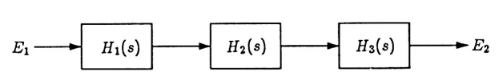
\includegraphics[scale=0.7]{./billeder/Kaskade}
	\caption{Kaskade af flere butterworth filtre.}
	\label{fig::anfilter_kask_butterworth}
\end{figure}
\FloatBlock

For at simplificere udregningerne vil alle operationsforstærkere anses for at være ideelle og arbejde i den lineær region, hvilket medfører $V_+ = V_-$.

\subsubsection{Trin 1} 
Det første trin i filteret er et 1. ordens butterworth filter og det designes ud fra ligning \ref{eq::filter_trin1},
\begin{equation}
	f_c = \dfrac{1}{2\cdot\pi\cdot R C} \label{eq::filter_trin1}
\end{equation} 	
hvor knækfrekvensen, $f_c$, er sat ved $17kHz$.
R9 vælges til $10K\Omega$ og C8 udregnes til $940pF$.

\begin{figure}[h]
	\centering
	\subbottom[]{%
		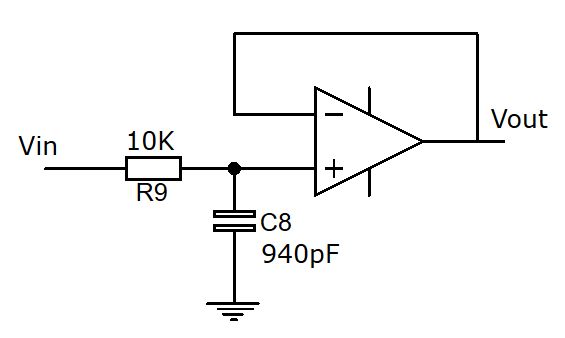
\includegraphics[width=6cm]{billeder/stage1a.png}
		\label{Trin 1 filter opbygning.}}
	\subbottom[]{%
		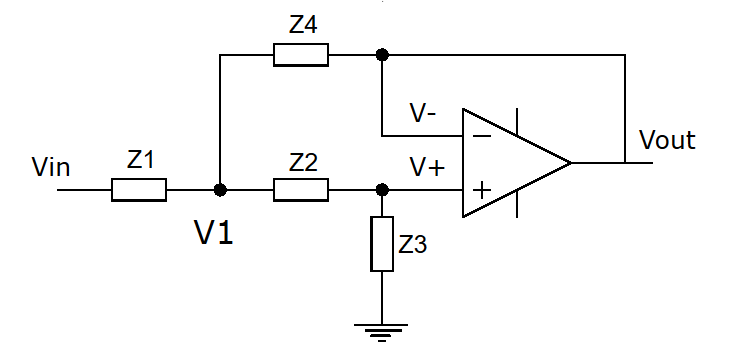
\includegraphics[width=6cm]{billeder/komp_udregn}
		\label{fig::anfilter_gensallen}}
	\caption{(a) Trin 1, filter opbygning. (b) Trin 2, Standard Sallen-Key filter.}
\end{figure}

\subsection{Trin 2}\label{sec::stage2}
Hvis kredsløbet på figur \ref{fig::anfilter_gensallen} betragtes, ses det at $V_+ = V1\dfrac{Z3}{Z2+Z3}$.

Ved Kirchoff's spændingslov findes\\
\begin{equation}
	\dfrac{V_{out}}{V_{in}} = \dfrac{V_{in}-V_1}{Z_1} = \dfrac{V_1 - V_{out}}{Z_4}+\dfrac{V_1}{Z_2+Z_3}
\end{equation}
Ved omrokering af disse ligninger findes

\begin{equation}\label{eq::anfilter_kcl}
	\dfrac{V_{out}}{V_{in}} = \dfrac{1}{\dfrac{Z_1Z_2}{Z_3Z_4}+\dfrac{Z_1}{Z_3}+\dfrac{Z_2}{Z_3}+1} = \dfrac{Z_3Z_4}{Z_1Z_2+Z_1Z_4+Z_2Z_4+Z_3Z_4}
\end{equation}

Standard formlen\footnote{Ligning 10.2 \cite[s. 218]{Su2002}}
 for et 2. ordens lavpas filter er
\begin{equation}\label{eq::anfilter_stndHS}
H(s) = \dfrac{Gw_0^2}{s^2 + \left(\dfrac{w_0}{Q}\right)s+w_0^2}
\end{equation}
Komponenter indsættes som følgende,
\begin{center}
	$Z_1 = R_{11}, \hspace{3mm} Z_2 = R_{12}, \hspace{3mm} Z_3 = \dfrac{1}{sC_{11}}$ \hspace{0.5mm} og \hspace{0.5mm} $Z_4 = \dfrac{1}{sC_{10}}$
\end{center}

Ud fra ligning \ref{eq::anfilter_kcl} fås overføringsfunktionen


\begin{equation}
H(s) = \dfrac{1}{s^2(C11C10R11R12)+s(C10R11+C10R12))+1}
\label{eq::SallenKey}
\end{equation}
 
Ud fra standard ligningen \ref{eq::anfilter_stndHS}, udledes,

\begin{equation}
	 C10(R11+R12) = \dfrac{1}{w_0 Q} \hspace{1cm} C11  C10  R11  R12 = \dfrac{1}{w_0^2} \nonumber
\end{equation}
hvor $Q = \dfrac{\sqrt{b_0}}{b_1}$ og $w_0 = 2\pi f_c$, og komponenterne R11 og R12 vælges til $32\si{\kilo\ohm}$. Ud fra to ligninger med to ubekendte, udregnes C10 udregnes til $940\si{\pico\farad}$, og C11 til at være $90 \si{\pico\farad}$.
\subsection{Trin 3}
Ud fra formel \ref{eq::SallenKey} udregnes også trin 3. Her vælges R16 til at være $150\si{\kilo\ohm}$ og C15 til at være $940\si{\pico\farad}$, C16 udregnes til at være $95\si{\pico\farad}$ og R15 til $6 \si{\kilo\ohm} $. 

\begin{figure}[h]
	\centering
	\subbottom[]{%
		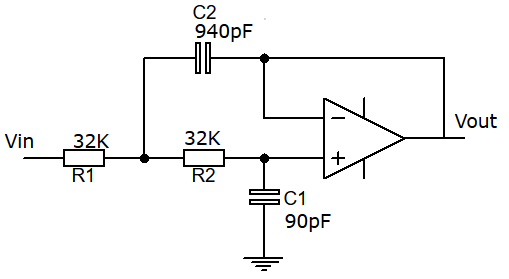
\includegraphics[width=0.4\textwidth]{./billeder/stage2a.png}
		\label{fig::anfilter_restage2}}
	\subbottom[]{%
		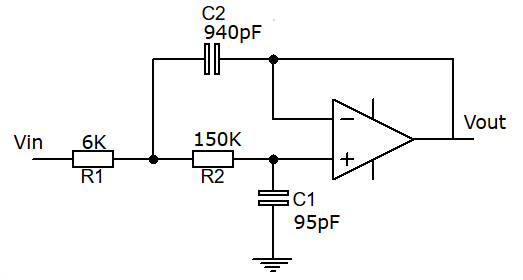
\includegraphics[width=0.4\textwidth]{./billeder/stage3a.png}
		\label{fig::anfilter_restage3}}
	\caption{(a) Trin 2 filter. (b) Trin 3 filter.}
\end{figure}
\FloatBlock

\subsection{DC Offset}
Da microcontrolleren ikke kan registrere negative signaler er det hensigtsmæssigt af påføre indgangssignalet et DC offset. Arbejdspunktet vælges til at være halvdelen af forsyningsspændingen. Dette opnås ved hjælp af kredsløbet på figur \ref{fig::anfilter_off}. \\
Dette DC offset betyder også at operationsforstærkerne i det analoge filter kun behøver en positiv forsyningsspænding. \\
På udgangen af rekonstruktionsfilteret placereres en kondensator pr. kanal for at eliminere dette DC offset og få et arbejdspunkt ved 0V.\\
I offset kredsløbet vil C3 og R3 generere et højpas filter. C3 udregnes, ud fra ligning \ref{eq::filter_trin1}, således at højpas filteret har en knækfrekvens ved 15Hz. C3 udregnes til at være $318\si{\nano\farad}$\\
Ligeledes vil kondensatoren placeret efter rekonsutruktions filteret, sammen med line-in impedansen generere et højpas filter. Line-in impedansen er defineret til $10\si{\kilo\ohm}$. Ligeledes med en knækfrekvens valgt til 15Hz, udregnes kondensatoren til $1.06\si{\micro\farad}$.

\begin{figure}[h!]
	\centering
	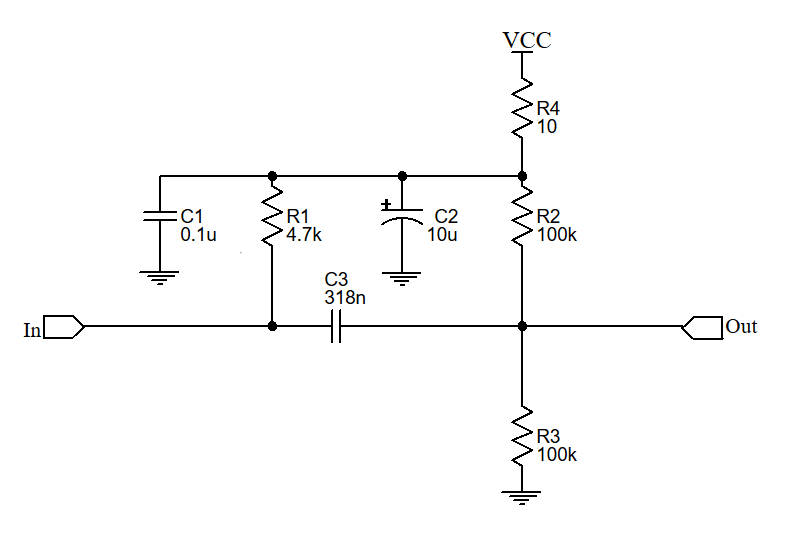
\includegraphics[scale = 0.35]{./billeder/offset.png}
	\caption{Kredsløbet for DC offset}
	\label{fig::anfilter_off}
\end{figure}







\subsection{Simulering}
Simuleringen af AA filteret er udført med simuleringsværktøjet LTspice \footnote{http://www.linear.com/solutions/ltspice}. Som det ses på figur \ref{fig::anfilter_aasim}, findes en dæmpning på -3dB ved 17kHz og en dæmpning på -12dB ved 22.5kHz. Forskellen i gruppeløbetiden er maksimalt $18 \si{\micro \second}$.

\begin{figure}[h!]
	\centering
	\subbottom[]{%
	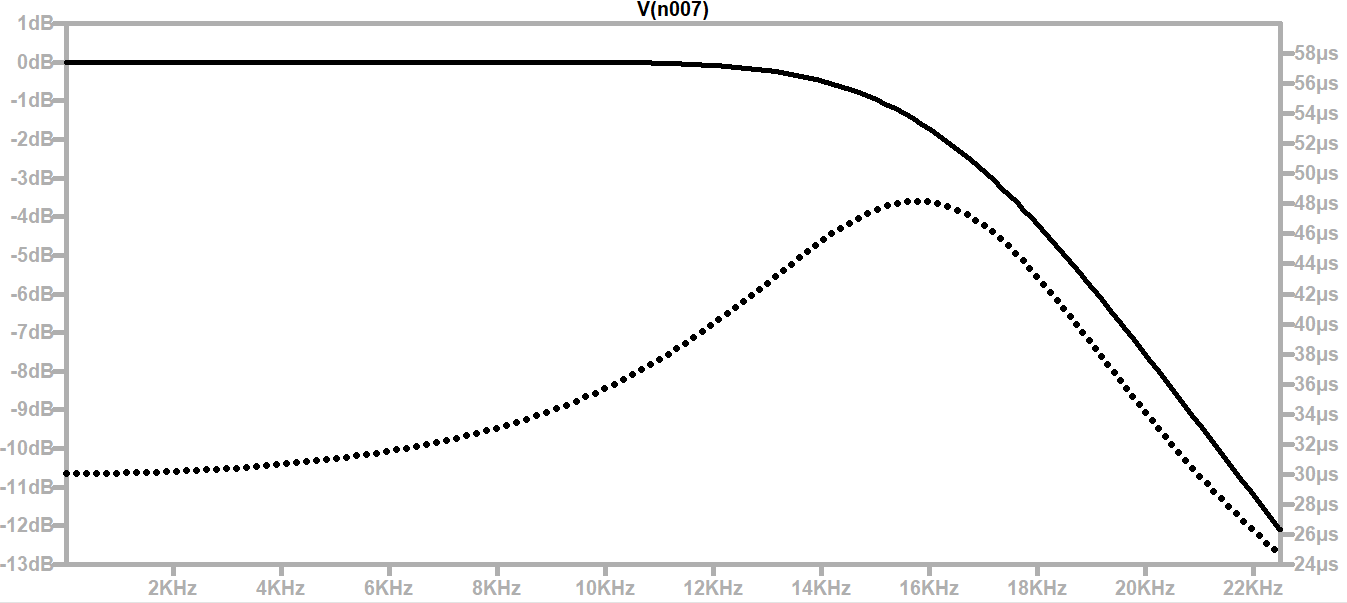
\includegraphics[width=0.48\textwidth]{./billeder/aa_sim1}
	\label{fig::anfilter_aasim}}
	\subbottom[]{%
	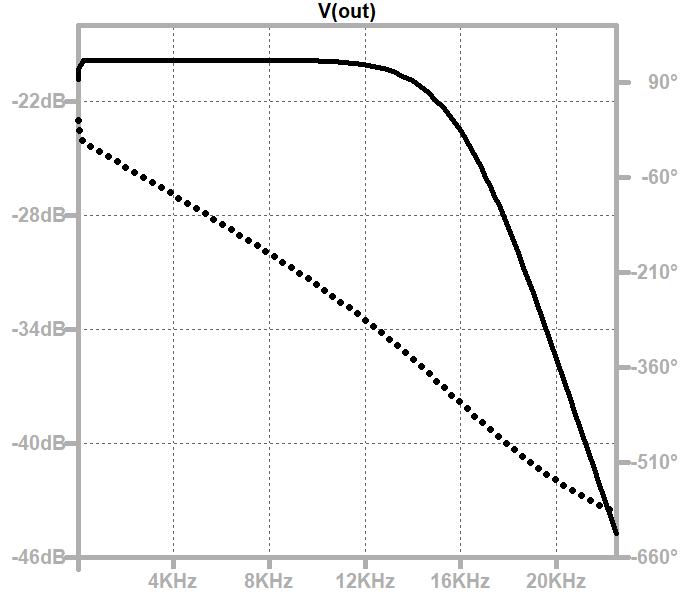
\includegraphics[width=0.48\textwidth]{./billeder/simtot.png}
	\label{fig::anfilter_sim_total}}
	\caption{(a) Simulering af AA filteret. Solid: Amplitude, Stiplet: Gruppeløbetid. \newline (b) Simulering af det samlede system. Solid: Amplitude, Stiplet: Fase.}
\end{figure}
\FloatBlock
Denne kaskade af filtre vil generere 5 poler. En reel pol i stage 1, to komplekse poler i stage 2 og to komplekse poler i stage 3. Disse kan ses i figur \ref{fig::anfilter_pol}.

\begin{figure}[h!]
	\centering
	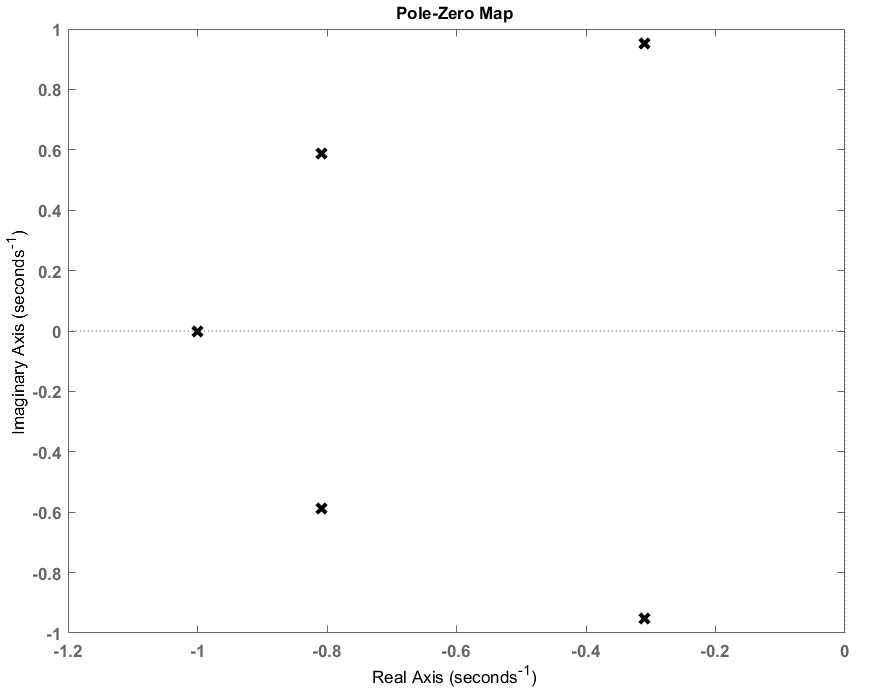
\includegraphics[scale = 0.35]{./billeder/pzmap}
	\caption{Kortlægning af polerne i AA og rekonstruktions filterne.}
	\label{fig::anfilter_pol}
\end{figure}
\FloatBlock
\section{Rekonstruktions filter}
\subsection{Formål}
I et system med både analoge og digitale signaler, bruges et rekonstruktionsfilter (også kaldet anti image filter) til at generere et "glat"  analogt signal ud fra f.eks. en DAC's udgangssignal. Et digitalt lydsignal har bølgeform som et trappetrin og indeholder en del højfrekvente komposanter, også kaldet "images". Et rekonstruktionsfilter konstruerer en mere udglattet version af det originale signal.
\subsection{Parametre og udregning}
Det er almindelig praksis at benytte et filter til rekonstruktion, magen til det filter der anvendes til antialiasing. For udregninger henvises til afsnit \ref{sec::anfilter_sallenpara}.

\subsection{Test og målinger}
På figur \ref{fig::anfilter_sim_total} ses amplitude og fase karakteristikken udfærdiget ved simulering af det samlede system. Bemærk faldet i amplitude ved lave frekvenser.

På figur \ref{fig::anfilter_recon} ses udgangssignalet fra DAC (gul), og det rekonstrueret signal (blå).
\begin{figure}[h!]
	\centering
	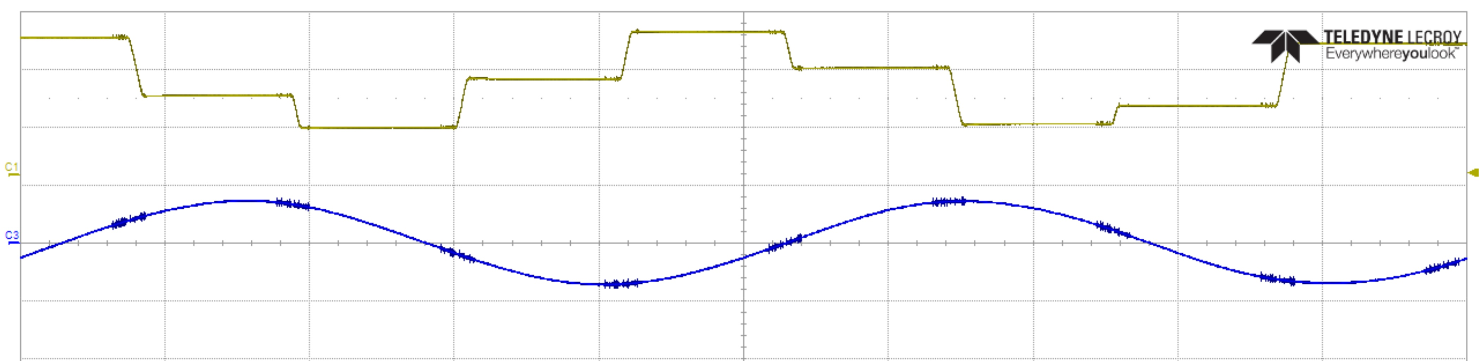
\includegraphics[scale = 0.4]{./billeder/reconstruction}
	\caption{Rekonstruktion af udgangen på DAC}
	\label{fig::anfilter_recon}
\end{figure}
\FloatBlock


Det kan ses på figur \ref{fig::anfilter_recon} at signalet fra rekonstruktions filteret indeholder højfrekvens støj. Dette kan skyldes kommunikation mellem Tiva-boardet og DAC'en\footnote{Se afsnit om SPI i afsnit 4.6}. \\
Dette kan løses ved at lave et højfrekvent lavpas filter, så tæt på udgangen som muligt. Der vælges et RC-led med en knækfrekvens på $1\si{\mega\hertz}$. Ligning \ref{eq::filter_trin1} benyttes, R sættes lig $88\si{\kilo\ohm}$ og $f_c = 1\si{\mega\hertz}$. C udregnes til $1.8\si{\pico\farad}$. I figur \ref{fig::anfilter_hf} ses signalet før og efter filteret.



\begin{figure}[h!]
	\centering
	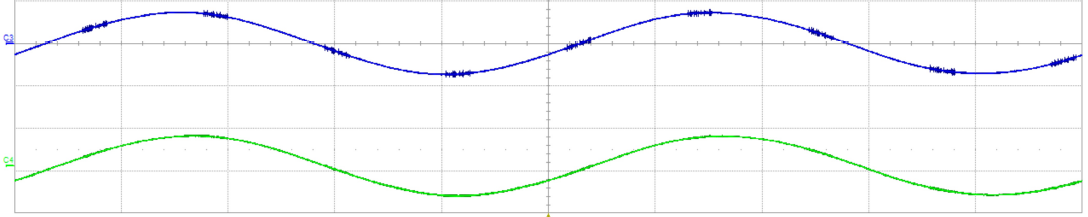
\includegraphics[scale = 0.55]{./billeder/hf.png}
	\caption{Udgangssignal før (blå) og efter (grøn) højfrekvens filter.}
	\label{fig::anfilter_hf}
\end{figure}
\FloatBlock

\subsection{Delkonkussion}
Det kan ses ud fra simuleringer at udregningerne af filtret har været tilfredstillende. De parametre der blev sat i afsnit \ref{sec::anfilter_sallenpara} er blevet overholdt. Efter realisering på pcb board kan der  ydermere konstateres at lydsignalet går igennem uden nævneværdige tab i øvre og lavere del af frekvensspektrumet. Test af filtrene kan ses i kapitel 6. Her ses det at amplituden passer overens med simulering, men at fasedrejningen er omkring $100 \si{\celsius}$ forkert. En stor del af denne fejl er grundet forsinkelser genereret af microcontrolleren, kommunikation til DAC og selve DAC'en. Dette diskuteres yderligere i kapitel \ref{kap:diskussion}.